\documentclass[a4paper]{article} % Specify A4 paper size
\usepackage[a4paper, margin=1in]{geometry} % Adjust margins for A4 paper
\usepackage{amsmath} % Add functionality for mathematical equations
\usepackage{graphicx} % For including images
\usepackage{pgf-pie} % For drawing pie charts
\usepackage{pgfplots} % For plotting charts

\title{A Comprehensive Sample Document} % Sets article title
\author{Amal Jose} % Sets author's name
\date{\today} % Sets date for date compiled

\begin{document} % Start of the document
    \maketitle % Creates title using information in the preamble
    
    \section{Introduction}
    Albert Einstein (1879–1955) was a theoretical physicist widely recognized as one of the greatest minds in history. 
    His groundbreaking theory of relativity revolutionized our understanding of space, time, and gravity. 
    Einstein's famous equation, $E=mc^2$, established the relationship between mass and energy, paving the way for modern physics and influencing technologies like nuclear energy. 
    He received the Nobel Prize in Physics in 1921 for his explanation of the photoelectric effect, a crucial step in developing quantum theory.
    
    Einstein was also known for his advocacy of civil rights, pacifism, and a passion for music. His legacy continues to inspire scientists and thinkers across the world.

    \section{Mathematical Expressions}
    Mathematics is a crucial aspect of academic writing. Here is an example of inline math: $E = mc^2$, and here is a displayed equation:
    \begin{equation}
        \int_a^b x^2 \, dx = \frac{b^3}{3} - \frac{a^3}{3}
    \end{equation}
    Equations like these can be used to demonstrate various mathematical concepts.

    \section{A Small Table}
    Tables are a great way to organize and present data. Below is an example:
    \begin{table}[h!]
        \centering
        \begin{tabular}{|c|c|c|}
            \hline
            \textbf{Category} & \textbf{Value} & \textbf{Percentage} \\ \hline
            Category A & 50 & 25\% \\ \hline
            Category B & 70 & 35\% \\ \hline
            Category C & 80 & 40\% \\ \hline
        \end{tabular}
        \caption{Sample Table of Categories}
        \label{tab:sample}
    \end{table}

    \section{A Pie Diagram}
    Pie charts visually represent data distributions. Below is a sample pie chart:
    \begin{figure}[h!]
        \centering
        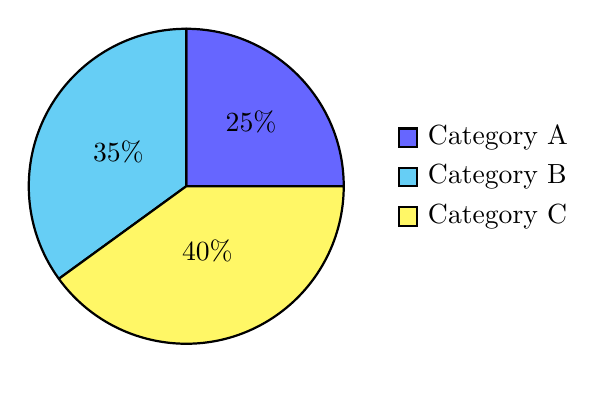
\begin{tikzpicture}
            \pie[text=legend, radius=2]{
                25/Category A,
                35/Category B,
                40/Category C
            }
        \end{tikzpicture}
        \caption{Sample Pie Chart}
        \label{fig:piechart}
    \end{figure}
    
    \section{A Parabola Chart}
    Below is a parabola chart showcasing the equation $y = x^2$:
    \begin{figure}[h!]
        \centering
        \begin{tikzpicture}
            \begin{axis}[
                axis lines = middle,
                xlabel = $x$,
                ylabel = {$y = x^2$},
                width=0.8\textwidth,
                height=0.4\textheight
            ]
                \addplot[
                    domain=-2:2, 
                    samples=100, 
                    color=blue,
                ]{x^2};
            \end{axis}
        \end{tikzpicture}
        \caption{Parabola Chart for $y = x^2$}
        \label{fig:parabola}
    \end{figure}

    \section{Conclusion}
    In this document, we explored how to use \LaTeX{} to create a well-structured and visually appealing document. 
    With sections on Albert Einstein, mathematical expressions, tables, and diagrams, we demonstrated the versatility of \LaTeX{} for academic and professional writing.

    \section*{References}
    \begin{enumerate}
        \item Lamport, L. (1994). \textit{\LaTeX: A Document Preparation System}. Addison-Wesley.
        \item Einstein, A. (1905). On the Electrodynamics of Moving Bodies. \textit{Annalen der Physik}.
        \item Kopka, H., \& Daly, P. W. (2003). \textit{Guide to \LaTeX}. Addison-Wesley.
    \end{enumerate}

\end{document}
